\section{Zero-Knowledge Proof (ZKP)}

If we focus solely on the final encrypted routing information ($\beta$), we can simplify the diagram from Figure \ref{fig:header_cipher} to the representation in Figure \ref{fig:schema_final_header}.
\footnote{It is important to note that Figure \ref{fig:schema_final_header} shows the final representation of the encrypted routing information, not the computation, as the integrity tags ($\gamma$) still need to be computed.}
We observe that a small part of the header contains the destination address ($\delta$) XORed with part of each shared secret. 
In other words, a substring $\beta^*$ of the final header is equal to $\Delta \xor h(s_3) \xor h(s_2) \xor h(s_1)$.

\begin{figure}[H]
    \centering
    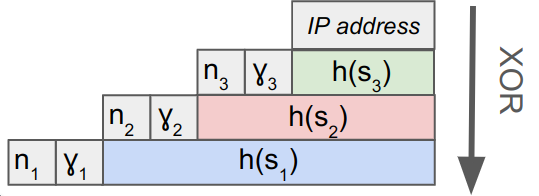
\includegraphics[width=0.5\linewidth]{Images/structure_final_header.png}
    \caption{Representation of the final encrypted routing information ($\beta$)}
    \label{fig:schema_final_header}
\end{figure}

Therefore, to user could prove that the destination address used in the original header is indeed the one he is authorized by its credentials (i.e. to one linked to its credential) without revealing anything about neither the destination, neither the routing path. 
In other words, proving that the $\Delta$ linked to the credential is the one used in $\beta^*$ = $\Delta \xor h(s_3) \xor h(s_2) \xor h(s_1)$.
To recall, with the current Sphinx mixnet architecture, a user can specify any destination address $\Delta$, and the packet will still traverse the entire mixnet before the fraud is detected at the exit gateway.

\paragraph{Idea} Proving that the address $\Delta$ from the credentials is indeed the one used in the header (i.e. $\beta^* = \Delta \xor h(s_3) \xor h(s_2) \xor h(s_1)$).

\paragraph{Limitations} Zero-Knowledge proofs are efficient with addition and multiplication operators, but not with the XOR (bitwise) operator, as XOR requires a separate proof for each bit instead of a single proof for the entire operation.

\paragraph{Solutions} To improve the efficiency of the ZKP proof, we could replace the XOR in the original schema (Figure \ref{fig:header_cipher}) with modular addition, measuring performance improvement, and ensuring it does not compromise security.

\paragraph{Discussion} If a user want to exhaust mixnode computation, he can provide the right $\Delta$ with a wrong $h(s_3)$. 
This strategy would exhaust the computational resources of the first two mixnodes before being detected at the third one, just before the exit gateway (one hop earlier that previously).
Thus we should look at a way to proof that $h(s_3)$ is correct as well... % ECC schema, Homomorphic Hash, in the construction of mixnode key that could be verified ???
Otherwise, we can think of it differently. 
Is it really a problem if user exhaust mixnodes computation ? 
It depends, in case of light network traffic is not a big deal since it follows the role of 'dummy' packet, improving the anonymity.
